\documentclass{article}
\usepackage{a4wide}


\usepackage{polski}
\usepackage[utf8x]{inputenc}
\usepackage{graphicx}
\usepackage{float}
\usepackage{hyperref}
\usepackage{listings}
\usepackage{mathtools}
\usepackage{amsmath}
\usepackage{hyperref}
\usepackage[margin=1in]{geometry}

\author{Lev Sergeyev}
\title{ZAPDC. Ćwiczenie 2. Interpolacja metodą dwuliniowa i metodą „najbliższego sąsiada”}

\date{ }
\begin{document}

\maketitle

%\pagebreakmovie15

\section{Przebieg ćwiczenia}
Za pomocą śródowiska Matlab zaprojektowałem 6 funkcji które pozwalają na zmianę rozmiarów obrazu cyfrowego za pomocą 3 algorytmów interpolacji:
\begin{itemize}
    \item Funkcję zmiany rozmiaru i proporcji obrazu:
	\begin{itemize}
		\item "nearest", interpolacja funkcją prostokątną
		\item "bilinear", interpolacja funkcją trójkątną
		\item "keys", interpolacja funkcją Keysa
	\end{itemize}
    \item Odpowiedniki poprzednich 3 funkcji, dokonują zmiany obrazu za pomocą wektoru(pozwala na zmianę rozmiaru, proporcji, obrotu, odbicia lustrzanego):
	\begin{itemize}
		\item "v\_ nearest"
		\item "v\_ bilinear"
		\item "v\_ keys"
	\end{itemize}
\end{itemize}

\section{Czas działania}
Dla jednego obrazu przeprowadzono 6 serii interpolacji dla każdej z 6 funkcji. Zmierzono czas działania funkcji. Następnie z otrzymanych wyników została wyliczona średnia. Czas podany w sekundach.
\begin{center}
    \begin{tabular}{ | c | c | c | c |}
    \hline
    Funkcja &  Skalowanie & Skalowanie + obrót  & Złożoność \\ \hline

     nearest  & 0.5847 & 2.5189 & \( O( (n^2) ^2 ) \)
    \\ \hline


     bilinear  & 3.4955 & 9.1013 & \( O( (n^2) ^4 ) \)
    \\ \hline
    
    
    
     keys & 11.6204 & 27.9314 & \( O( (n^2) ^6 ) \)
    \\ \hline

    \end{tabular}
\end{center}

\pagebreak

\section{Porównywanie otrzymanych obrazów}

\subsection{Piksele}
Zmiana rozmiaru: \\
\(Lx = 32 Lx_0\) \\
\(Ly = 32 Ly_0\) \\
\begin{center}
    \begin{tabular}{ | p{2cm} | c |}
    \hline
    Funkcja &  Obraz \\ \hline
    
    \smallskip oryginał & 
    \raisebox{-\totalheight}{\scalebox{2}{
\includegraphics{img/pixels.png}}}
     \\ \hline

    \smallskip nearest  & 
    \raisebox{-\totalheight}{\scalebox{0.5}{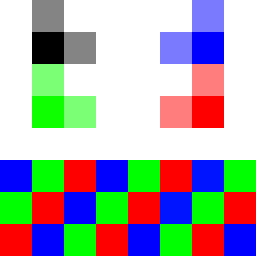
\includegraphics{img/pixels_n.png}}} 
    \\ \hline

    \smallskip bilinear  & 
    \raisebox{-\totalheight}{\scalebox{0.5}{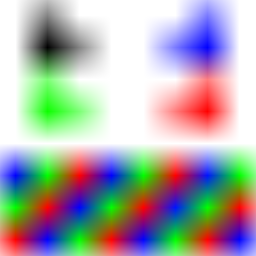
\includegraphics{img/pixels_b.png}}} 
    \\ \hline
    
    \smallskip keys & 
    \raisebox{-\totalheight}{\scalebox{0.5}{
\includegraphics{img/pixels_k.png}}} 
    \\ \hline
    \end{tabular}
\end{center}

\pagebreak

\subsection{Jabłko}
Wektorowe funkcje interpolujące: \\
\(Lx = -2.5 Lx_0\) \\
\(Ly = 1.5 Ly_0\) \\
\( \Phi_{rot} = -10^\circ \)  \\
\begin{center}
    \begin{tabular}{ | p{2cm} | c |}
    \hline
    Funkcja &  Obraz \\ \hline
    
    \smallskip oryginał & 
    \raisebox{-\totalheight}{\scalebox{1.5}{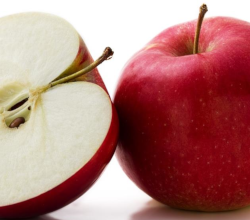
\includegraphics{img/jab_s.png}}}
     \\ \hline


    \smallskip nearest  & 
    \raisebox{-\totalheight}{\scalebox{0.3}{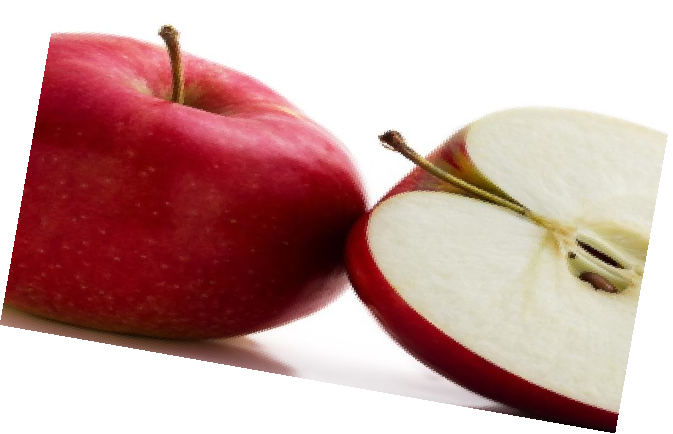
\includegraphics{img/jab_n.png}}} 
    \\ \hline


    \smallskip bilinear  & 
    \raisebox{-\totalheight}{\scalebox{0.3}{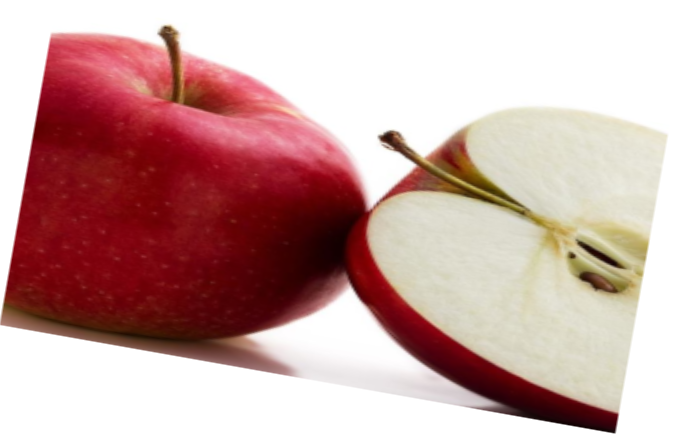
\includegraphics{img/jab_b.png}}} 
    \\ \hline
    
    
    
    \smallskip keys & 
    \raisebox{-\totalheight}{\scalebox{0.3}{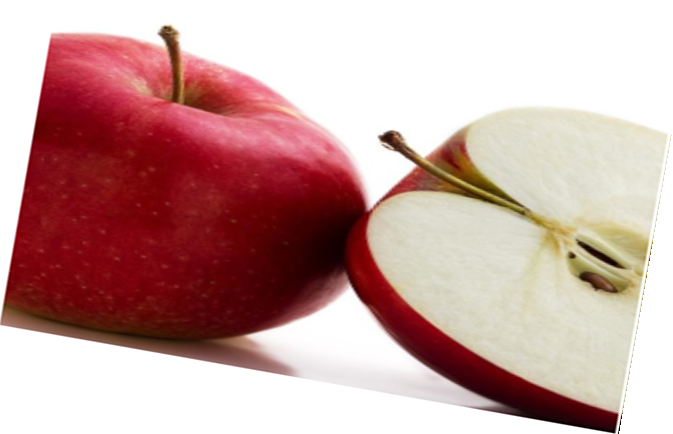
\includegraphics{img/jab_k.png}}} 
    \\ \hline

    \end{tabular}
\end{center}

\pagebreak

\subsection{Siatka}
\(Lx = 0.8 Lx_0\) \\
\(Ly = 0.8 Ly_0\) \\
\( \Phi_{rot} = 3^\circ\)  \\
\begin{center}
    \begin{tabular}{ | p{2cm} | c |}
    \hline
    Funkcja &  Obraz \\ \hline
    
    \smallskip oryginał & 
    \raisebox{-\totalheight}{\scalebox{0.5}{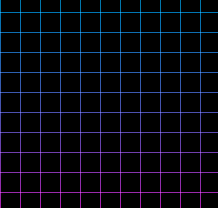
\includegraphics{img/grid_s.png}}}
     \\ \hline


    \smallskip nearest  & 
    \raisebox{-\totalheight}{\scalebox{0.5}{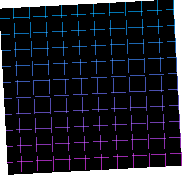
\includegraphics{img/grid_n.png}}} 
    \\ \hline


    \smallskip bilinear  & 
    \raisebox{-\totalheight}{\scalebox{0.5}{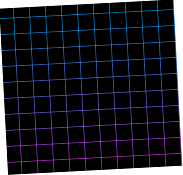
\includegraphics{img/grid_b.png}}} 
    \\ \hline
    
    
    
    \smallskip keys & 
    \raisebox{-\totalheight}{\scalebox{0.5}{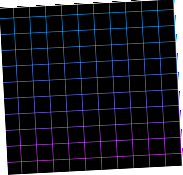
\includegraphics{img/grid_k.png}}} 
    \\ \hline

    \end{tabular}
\end{center}

\section{Wnioski}
\par
Porównując skalowane obrazy można dojść do wniosku, że największa dokładność należy do interpolacji funkcją prostokątną | metoda "najbliższego sąsiada". Dodatkowo, przez mniejszą złożoność obliczeniową, metoda "najbliższego sąsiada" jest najszybszym algorytmem do skalowania. 
\par
Funkcje liniowej interpolacji i Keys'a pozwalają otrzymać znacznie bardziej naturalny dla człowieka obraz po skalowaniu. Dokładne porównać te dwie funkcje można za pomocą skalowania obrazu "piksele": w wyniku skalowania interpolacją dwuliniową można zauważyć "liniowość" przejść w odróżnieniu od płynnych przejść (krzywą funkcji sześciennej) interpolacji Keys'a.\\
\par
Interpolacja funkcją Keysa może dać jakościowo najlepszy wynik, ale potrzebuje znacznie więcej czasu, który będzie wynosił \( {t_{nearest}}^3\) lub \({t_{bucubic}}^2\).
\par
Wadą interpolacji liniowej i Keys'a można nazwać rozmycia które mogą powstać na granicach objektów na obrazie po skalowaniu w górę.
Wadą interplolacji funkcją prostokątną można nazwać zjawisko aliasingu(widoczne na "siatka") po skalowaniu w dół.
\par
Często można zauważyć w aplikacjach do pracy z grafiką rastrową, że interpolacja najbliższym sąsiadem jest wykorzystywana dla szybkiego podglądu wyniku operacji skalowania, która następnie wykonywana jest bardziej złożonym algorytmem.

\end{document}
